\chapter{Hierarchical Approximate Convex Decomposition}\label{cha:meth2}
One of the go-to-methods for collision detection concerning complex concave objects
are convex decomposition. Dividing the concave model down into subsets, which are
all convex can give composite shapes that are concave yet still work with the
traditional collision detection and response models since they work on convex
sub-shapes, see figure~\ref{fig:hacdSimple}, where an initially concave shape has
been subdivided in smaller convex shapes.

\begin{figure}[H]
  \centering
  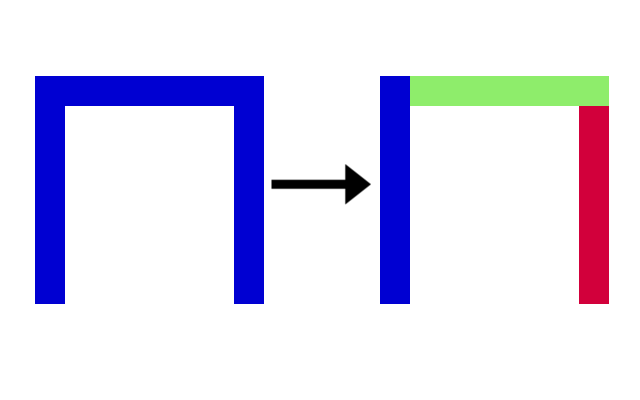
\includegraphics[width = 0.8\textwidth]{hacdSimple.png}
  \caption{The basic idea behind HACD, subdividing a concave shape into smaller convex ones.}
  \label{fig:hacdSimple}
\end{figure}

\section{Implementation}
Bullet 2.83 contain a
composite (or compound) shape, a shape container which contain sub-shapes and act
as a joint rigid body. Bullet updates the inertia of the object internally as
more sub-shapes are added, as well as the bounding box needed for the SAP.

An implementation of HACD is included with Bullet's source code and the code is
developed by Khaled Mamou. Some input parameters are available, these have been
left as the recommended parameters. The parameters control for instance, concavity
penalty weights, (i.e if you can disregard a small concavity)
and the maximum amount of points per convex hull.
The method while effective in terms of result can not be described as
particularly effective in terms of performance. A Utah Teapot of around 4300 vertices,
takes approximately 25 seconds to decompose. The method is in addition rotationally
 variant, so results may vary depending on the rotation of the object which is to be decomposed.
This is illustrated in figure~\ref{fig:HACD} and~\ref{fig:HACDrot}, where the later
 was rotated by 90 degrees prior to decomposition. While the difference is not
 major and will produce comparable results it is however clearly visible and should be kept in mind.
 The rotated decomposition also took somewhat longer to perform, about 29 seconds.

 \begin{figure}[H]
   \centering
   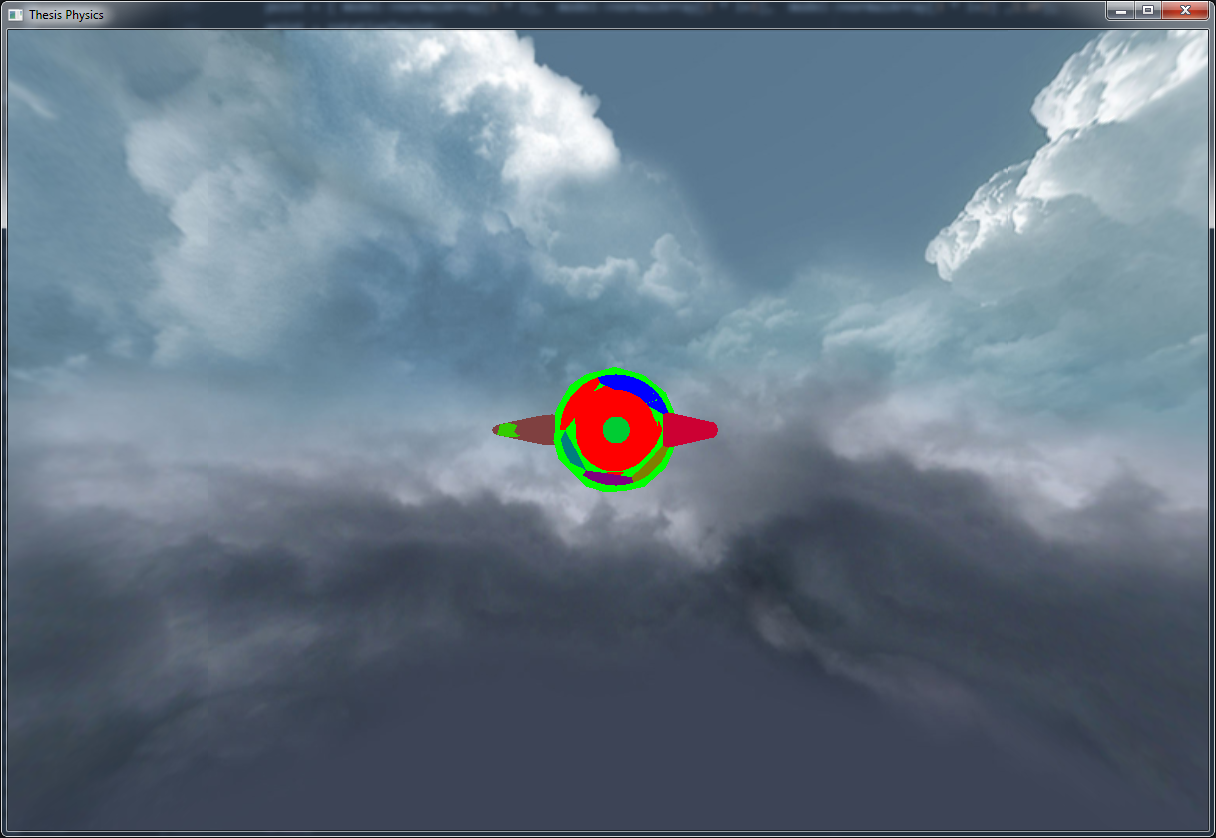
\includegraphics[width = 0.8\textwidth]{Screenshots/hacdTeaPot02-05.png}
   \caption{The decomposition from HACD method, model left in initial orientation.}
   \label{fig:HACD}
 \end{figure}

 \begin{figure}[H]
   \centering
   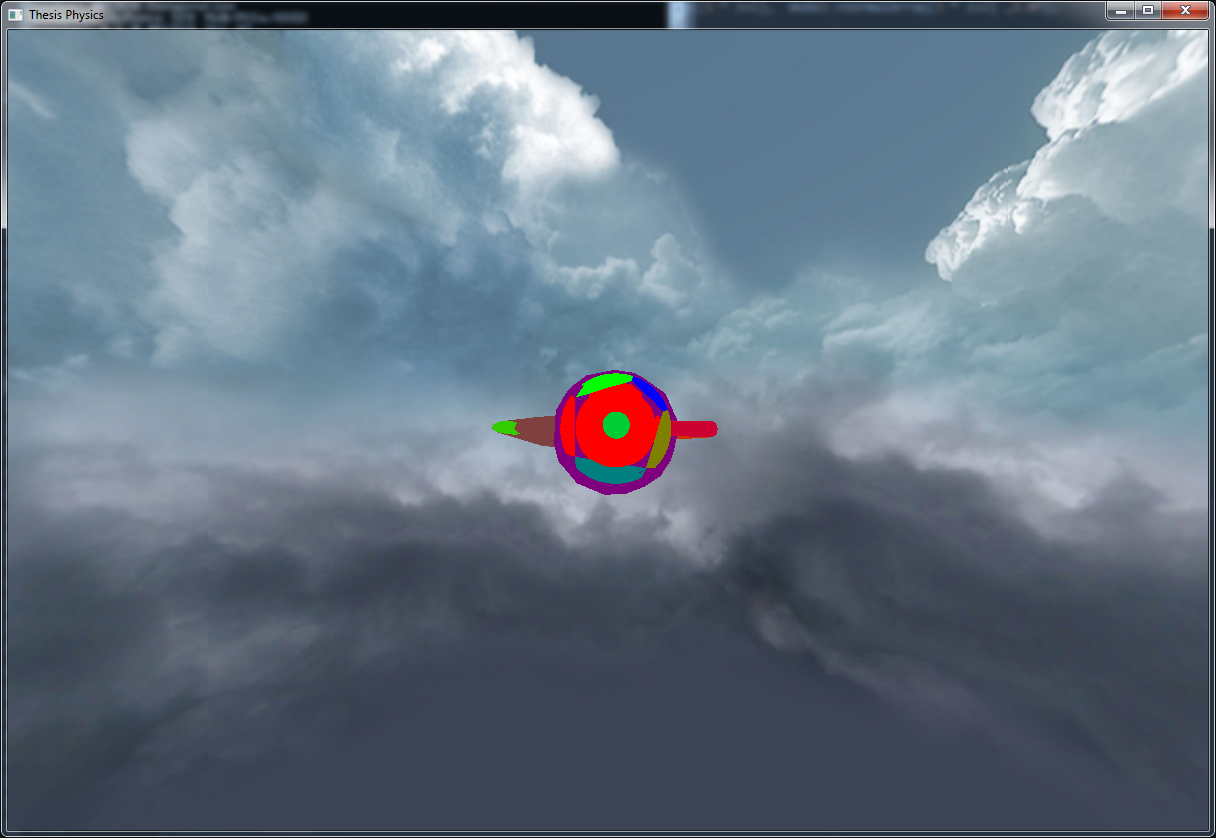
\includegraphics[width = 0.8\textwidth]{Screenshots/hacdRotatedTeaPot02-05.png}
   \caption{The decomposition from HACD method, model 90 degrees around z axis compared to initial orientation.}
   \label{fig:HACDrot}
 \end{figure}

Several instance of the rigid body can now be created and added in the same fashion
as in the case of the Axis-Aligned Bounding Rectangle, see chapter~\ref{cha:meth}.

The simulation takes approximately 3-4 times as long (sometimes up to 10 times)
 to run than the much simpler bounding rectangle method, but note that for this
 case there is now twelve models per teapot. Each convex hull consist of fifty
 to a hundred points. This makes for a quite more difficult task
to simulate. Disregarding the complexity of the hulls we still have twelve times
as many models being simulated. It is likely the broadphase that saves us from
experiencing further reductions in performance.

One can easily note that during a simulation much more time is spent in the last
part of the simulation when most of the models are quite stationary and only small
changes are made. It takes quite a lot of time for all the models to become
completely stationary. A lot of small rolling motions, likely due to the round
shape of the Utah Teapot can be observed.

\section{Testing}
For details on the parameters used in the tables presented in this section I
 refer to section~\ref{sec:testing}, in chapter~\ref{cha:meth} on
 page~\pageref{sec:testing}.

\section{Results}
Two of the simulations at scale factor 0.5, can be seen in figure~\ref{fig:hacd0.1}~and~\ref{fig:hacd0.0}. Where the first
is 'energy relaxed' (as described in section~\ref{sec:testing}) and the second is not.
The simulations took about 60 and 144 seconds respectively. The decomposition
time excluded since the sub models were read from file instead. One can note
that there is little qualitative difference in the distribution of the Utah Teapots
in the relaxed simulation versus the non-relaxed simulation.

\begin{figure}[H]
  \centering
  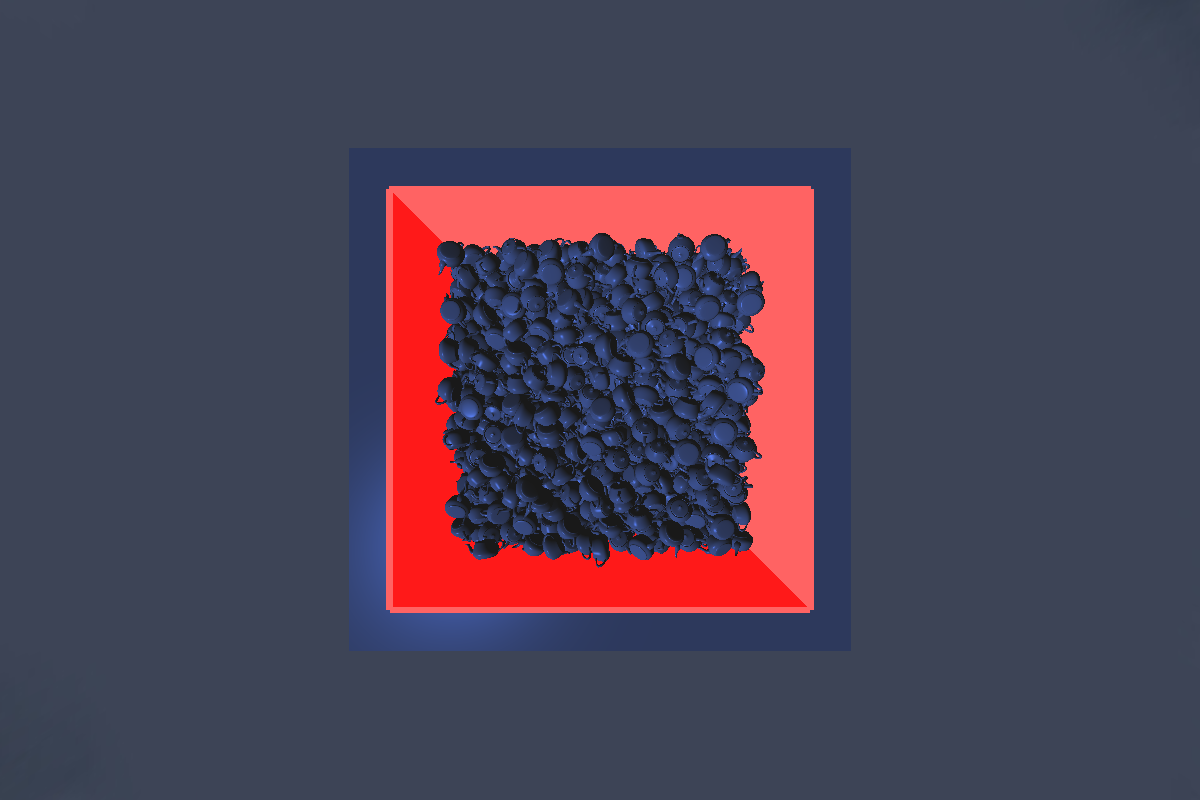
\includegraphics[width = 0.8\textwidth]{Screenshots/hacdResult01.png}
  \caption{The end result of the energy relaxed simulation}
  \label{fig:hacd0.1}
\end{figure}

\begin{figure}[H]
  \centering
  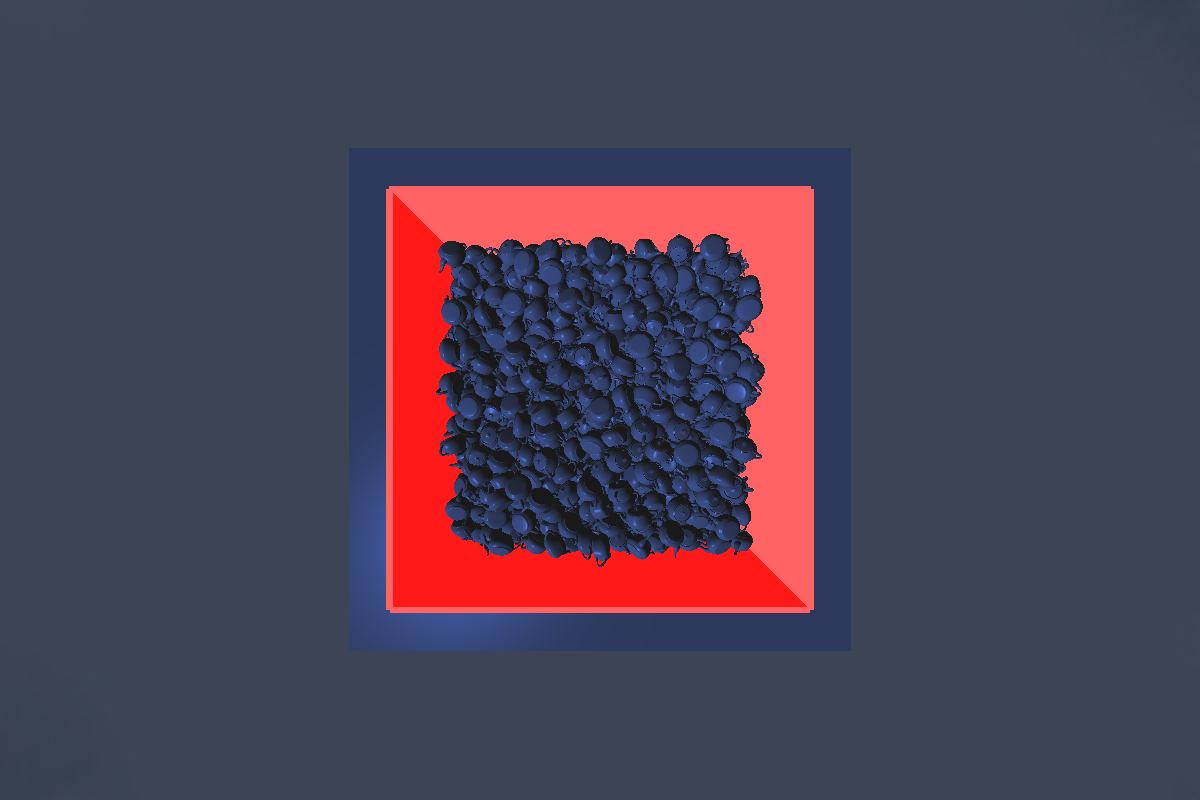
\includegraphics[width = 0.8\textwidth]{Screenshots/hacdResult0.png}
  \caption{The end result of the non-relaxed simulation}
  \label{fig:hacd0.0}
\end{figure}

\begin{figure}[H]
  \centering
  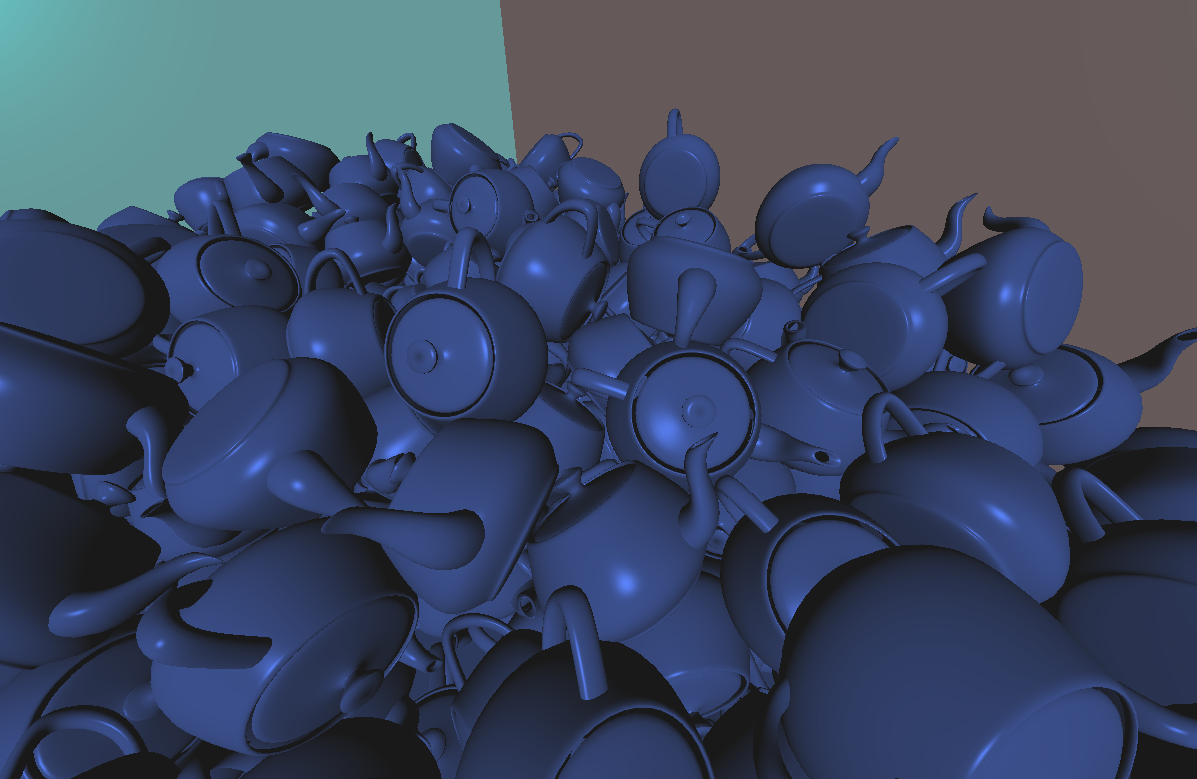
\includegraphics[width = 0.8\textwidth]{HACDtight.png}
  \caption{Close-up of finished result.}
\end{figure}

\section{Remarks}
The lack of performance for the decomposition itself is in this case something
which is not a huge problem as we have little need for it. The models are
decomposed at the start and copies of the same shape are used, i.e. no additional
HACD's are performed. The result were also saved to an obj file so easy and quick
 loading of the decomposed models could be used for the testing.

The performance for the whole system simulation, while not phenomenal, is fast enough
for the generation of synthetic data, granted that suitable simulation parameters
are selected, as can be seen in the tables presented above. Especially important
is the energy relaxation which helps the simulation times quite a bit.

As opposed to the Rectangle Bounding Box this method does handle concave models,
and the models generated from HACD is quite tight fitting.
%A concave collision result is portrayed in figure~\ref{fig:concaveHACD}.

\section{Limitations}
The limitations of this method are mainly concerning the performance. The fact
that the parameters of the HACD might affect the decomposition makes the system
as a whole less robust.
